\documentclass{article}
\usepackage{graphicx}
\usepackage{caption}
\usepackage{subcaption}
\usepackage{natbib}
\usepackage{hyperref}
\usepackage{amsfonts}
\usepackage{amsmath}

\begin{document}

\title{Efficient Gibbs Sampling for Image Models based on Fields of 
Experts}

\author{Jonas Arnfred}

\maketitle

\section{Introduction}

For a machine learning algorithm to have any practical use, it must 
produce good results and it must produce them fast. An algorithm with a 
high quality output will push the boundaries of what's possible, but if 
it isn't efficient the applications to real life situations become 
drastically limited.  Most people do not have days to wait for a 
simulation to be done, nor do they have a cluster of nodes to run the 
algorithm on, but what's more, many applications require a close to 
real-time output or work with input sizes drastically larger than the 
test examples used to demonstrate the algorithms.

The Field of Experts framework proposed in \citep{stefan} attempts to 
address both sides of the problem by simplifying expert models to use 
convolution filters making it feasible to sample images from a 
generative framework. The particular denoising algorithm proposed in 
\citep{uwe} makes use of these advantages to a large part, but in 
efforts to prove the worth of the Fields of Experts algorithm in terms 
of quality, they sacrifice efficiency to achieve the best possible 
result. This leaves it an open question whether Fields of Experts has 
the potential to reach a good compromise between speed and quality.

In this paper I try to explore how much we need to sacrifice in terms of 
quality in order to gain extra efficiency. Due to the limited scope of 
this project, this exploration is done entirely within the frame of an 
already learned image prior taken from \citep{uwe}. In the first part of 
this paper I analyse Fields of Experts to find the main efficiency 
bottlenecks and discuss what variables I can adjust in the hopes of 
seeing an increase in speed. In the second part I address this 
discussion and provide data for the behaviour of Field of Experts given 
the suggested adjustments.

\section{Method}

To analyse where the performance bottleneck is located in the Field of 
Experts, we need to take a look at how the prior is defined. According 
to \citep{stefan} and \citep{uwe} the framework is defined as follows: 
Given an image $\textbf{u} \in \mathbb{R}^n$, its probability density 
can be written as:

\begin{equation}
	p(\textbf{u}; \Theta) = 
	\frac{1}{Z(\Theta)}e^{-\epsilon||\textbf{u}||^2/2} \prod_{r=1}^{R} 
	\prod_{i=1}^{n} t_r(s_{ri})
\end{equation}

where $s_{ri}$ is the circular convolution of $\textbf{u}$ with the 
filter $f_r$, $r = 1, \ldots , R$, $\,\Theta$ is a collection of model 
parameters ($f_r, \alpha_r$, $\sigma_r$) and $Z$ is the partition 
function.  The potentials $t_r(s)$ used are mixtures of Gaussian defined 
as:

\begin{equation}
	t_r(s) = \sum_{j=1}^{J} \alpha_{rj}\mathcal{N}(s|o, \sigma^2_{rj})
\end{equation}

where $J$ is the number of mixtures used in the model, $\alpha_{rj}$ is 
the scale for the $j$th gaussian and $\sigma^2_{rj}$ the variance. To 
sample from this density \citep{uwe} propose using an auxiliary-variable 
Gibbs sampler which introduces indicator variables $z \in \left\{1, 
\ldots, J\right\}$ which selects the component of the Gaussian mixture.  
This way $t_r(s_{ri})$ given $z_{ri}$ is equivalent to a Gaussian and 
much easier to sample from. Using Gibbs sampling we can alternate 
between sampling $\textbf{z}^{(t + 1)} \sim 
p(\textbf{z}|\textbf{u};\Theta)$ and $\textbf{u}^{(t + 1)} \sim 
p(\textbf{u}|\textbf{z};\Theta)$ where t is the current iteration.  With 
a little restructuring of (1) and (2) the conditionals for $\textbf{u}$
and $\textbf{z}$ are given by

\begin{equation}
	p(z_{ri}|\textbf{u};\Theta) \propto \alpha_{rz_{ri}} \cdot 
\mathcal{N}(s|o, \sigma^2_{rz_{ri}})
\end{equation}

\begin{equation}
	p(\textbf{u}|\textbf{z};\Theta) \propto \mathcal{N}\left(\textbf{u}; 
	0, \left( \epsilon \textbf{I} + \sum_{i=1}^{R}B_r^T 
	diag(1/\sigma^2_{rz_{ri}}) B_r \right)^{-1} \right)
\end{equation}

where $B_r$ are the matrices such that $B_r \textbf{u} = \textbf{f}_r 
\star \textbf{u}$. If we denote $\,A = \epsilon \textbf{I} + 
\sum_{i=1}^{R} B_r^T diag(1/\sigma^2_{rz_{ri}}) B_r\,$ and define 
$\tilde{A} = (\textbf{I}/\sigma^2 + A^{-1})^{-1}$, the posterior for 
image denoising given the noisy image $\textbf{y}$ is given by:


\begin{align}
	p(\textbf{u}| \textbf{y}, \textbf{z}; \Theta) & \propto 
	p(\textbf{y}|\textbf{u}) \cdot p(\textbf{u}|\textbf{z};\Theta) \\
	& \propto \mathcal{N} \left( \textbf{u} ; \, \tilde{A} y / \sigma^2, 
	\, \tilde{A}\right)
\end{align}

To sample from $p(\textbf{u}|\textbf{z};\Theta)$ we sample $n_0 \sim 
\mathcal{N}(0, \textbf{I}) \in \mathbb{R}^{Rn}$. If we let $\,n_1 = 
\sum_{i=1}^{R} B_r^T diag(1/\sigma^2_{rz_{ri}})\,$ we can sample 
$u_{\delta} = A^{-1} n_1 \sim \mathcal{N}(0, A^{-1})$ and calculate 
$u_{\mu} = A^{-1} \textbf{y}/\sigma^2$. We then get our denoised image 
$\textbf{u} \sim \mathcal{N} \left(\tilde{A} y / \sigma^2, \, 
\tilde{A}\right)$ by adding $\textbf{u}_{\delta}$ and 
$\textbf{u}_{\mu}$.

This means that in order to sample from the posterior distribution we 
need to solve two linear systems: $\textbf{u} = \tilde{A}^{-1} \cdot 
n_1$ and $\textbf{u}_{\mu} = \tilde{A}^{-1} \cdot \textbf{y}/\sigma^2$.  
Since these two systems are solved for every iteration of the Gibbs 
sampling, they constitute the main perfomance bottleneck while denoising 
an image.  

\subsection{Optimizing for Conjugate Gradient}

The denoise algorithm proposed by \citep{uwe} uses choleski 
decomposition to solve the systems which doesn't scale well to images 
and doesn't provide much room for optimizations. The first step of 
speeding up the algorithm was thus to implement a Gibbs sampler that 
uses the conjugate gradient algorithm. This allowed for several possible 
ways to increase the speed of the algorithm: Preconditioning, lower 
error tolerance, resizing of the scales ($\sigma^2_{rz_{ri}}$) and 
finally eliminating the more extreme values of the scales.

Since the goal of the implemented denoising algorithm is not to achieve 
superior denoising results, but rather serve as a tool for analysis, my 
implementation differs from the one specified in \citep{uwe} on one 
account.  Instead of running four Gibbs samplers concurrently, only one 
sampler is run.  This makes it more difficult to estimate when to stop 
the algorithm, since it is not possible to use the variance in between 
the four concurrent samplers to estimate when they are converging stop.  
Instead I let the Gibbs sampler run for a set amount of conjugate 
gradient iterations.  This facilitates analysis since the accumulated 
amount of conjugate gradient iterations provides a common atomic unit 
across different runs.

In order to speed up conjugate gradient we can use a preconditioner to 
improve the condition number of a matrix $Q$. If are trying to solve the 
system $Qx = b$ and have a matrix $M$ for which $\kappa(M^{-1}Q) \ll 
\kappa(Q)$ then we can usually solve $Qx = b$ faster by solving 
$M^{-1}Qx = M^{-1}b$ instead \citep{pain}. The problem lies in finding 
an M which is invertible and in fact improves the condition number. For 
this project I've used the diagonal of $\tilde{A}$ in fourier space.

Alternatively we can increase how small the error must be before we stop 
iterating. This in turn means that we are accepting solutions that are 
further from the true solution of the system which might negatively 
impact the quality of the denoising.

It might also prove useful to change parameters to create equations that 
are faster to solve. One way to do this is by changing the scales used 
in the gaussian mixture. In \citep{uwe} a fixed number of 15 scales is 
specified as $s = exp(0, \pm1, \ldots, \pm5, \pm7, \pm9)$. To scale $s$ 
I introduce a factor $p \in \{1, .95, .9, \ldots , 0.1\}$ in $s = 
exp(\ldots)^p$. This ensures that the more extreme scales are altered 
more than those in between.
%
%
%
% What do I want to write about?  First introduce the probabilistic 
% Model, then
% shortly go over how the gibbs sampling works

% Now go into depth with the systems I need to solve to denoise an image 

% Now introduce the differences from DARMSTADT and specify on what points my
% solution is different from theirs (Don't talk about why)

% Related to differences, talk about using cg instead of cholesky
% decomposition, about using number of conjugate gradient iterations to
% measure out the burn-in time. About how I'm only sampling from one image and
% not 4 per iteration. About how I'm stopping the process after a fixed number
% of iterations too.  Also talk about the burn-in samples are discarded and
% that the average of the samples that follow is the basis for the image

% Now talk about the experiments: How was the data collected?
% Talk about exclusions of scales
% Talk about variations or scalings of scales
% Talk about variations in CG cut-off rate (tolerance)
% Mention that the data is for one image only, and not averaged

% Show plot of 5 images with different sigma noise

\section{Results}

\begin{figure}[h]
	\makebox[\textwidth][c]{%
		\begin{minipage}[b]{0.25\textwidth}
                \centering
				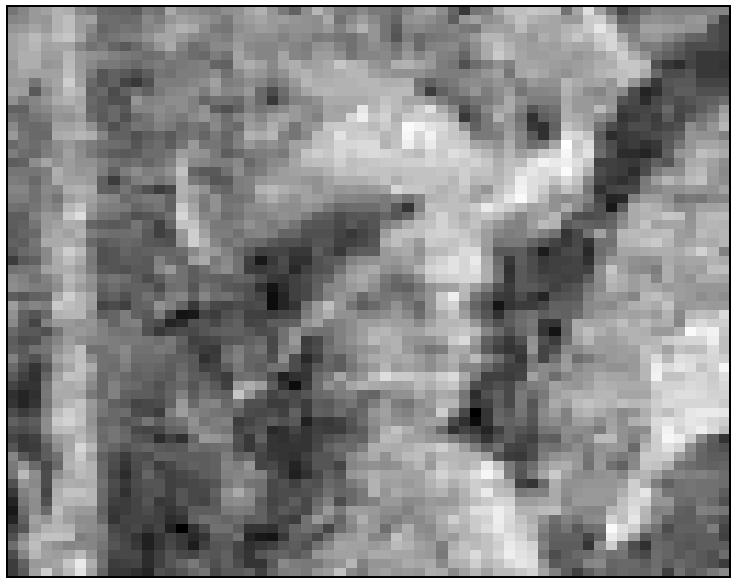
\includegraphics[width=\textwidth]{img/img_22_psnr}
				\small{psnr $\approx 22$}
				\label{psnr_22}
		\end{minipage}%
		~ %add desired spacing between images, e. g. ~, \quad, \qquad 
		\begin{minipage}[b]{0.25\textwidth}
                \centering
				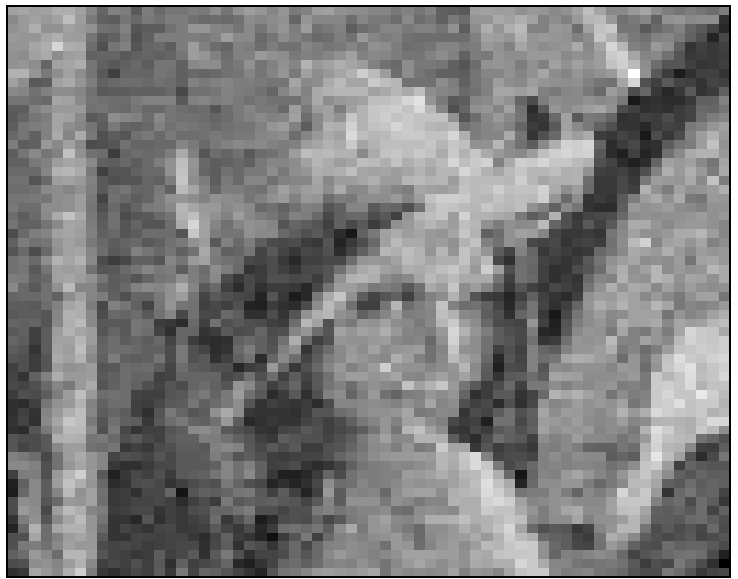
\includegraphics[width=\textwidth]{img/img_24_psnr}
				\small{psnr $\approx 24$}
				\label{psnr_24}
		\end{minipage}%
		~ %add desired spacing between images, e. g. ~, \quad, \qquad 
		\begin{minipage}[b]{0.25\textwidth}
                \centering
				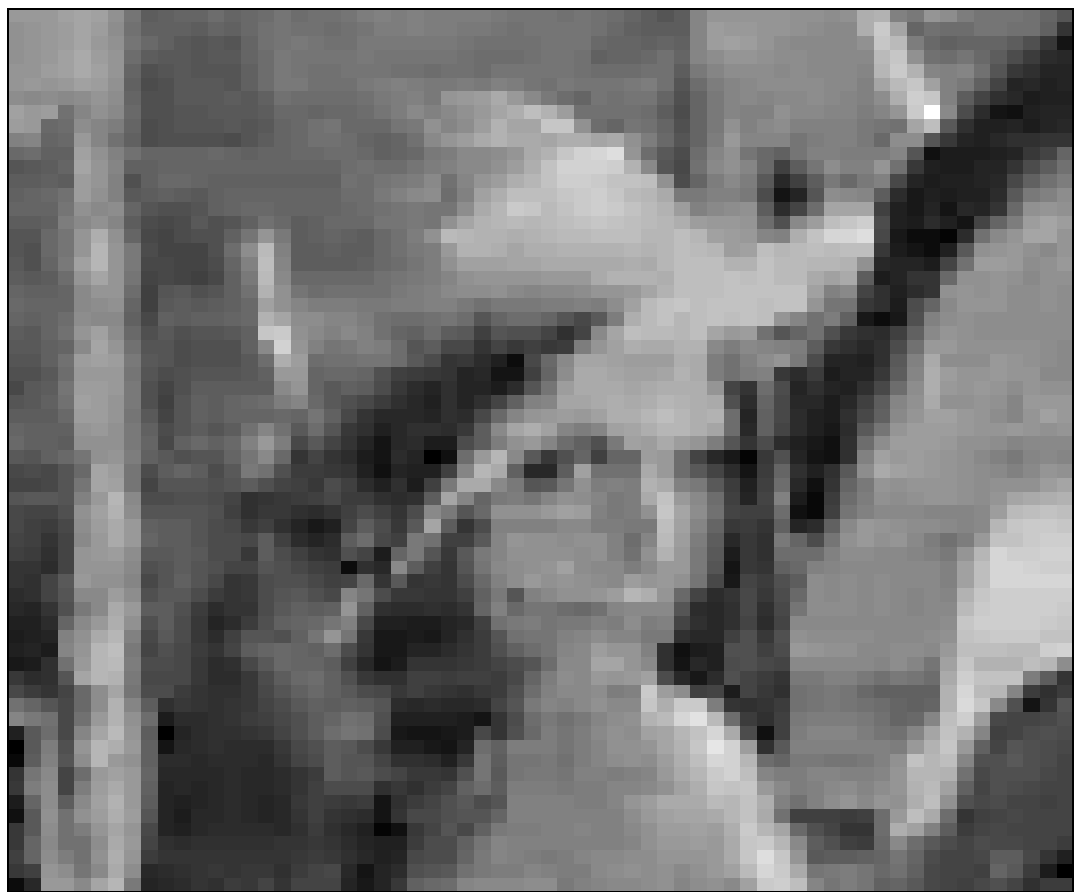
\includegraphics[width=\textwidth]{img/img_26_psnr}
				\small{psnr $\approx 26$}
				\label{psnr_26}
		\end{minipage}%
		~ %add desired spacing between images, e. g. ~, \quad, \qquad 
		\begin{minipage}[b]{0.25\textwidth}
                \centering
				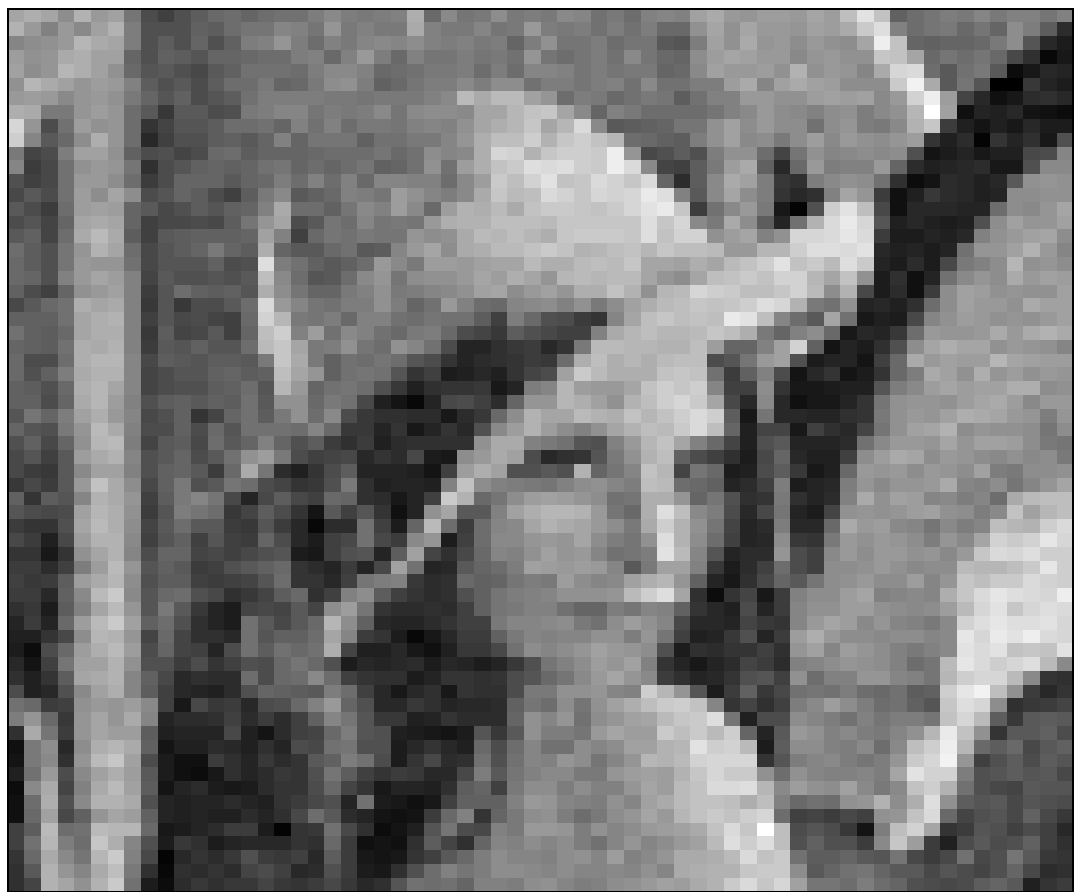
\includegraphics[width=\textwidth]{img/img_28_psnr}
				\small{psnr $\approx 28$}
				\label{psnr_28}
		\end{minipage}%
		~ %add desired spacing between images, e. g. ~, \quad, \qquad 
		\begin{minipage}[b]{0.25\textwidth}
                \centering
				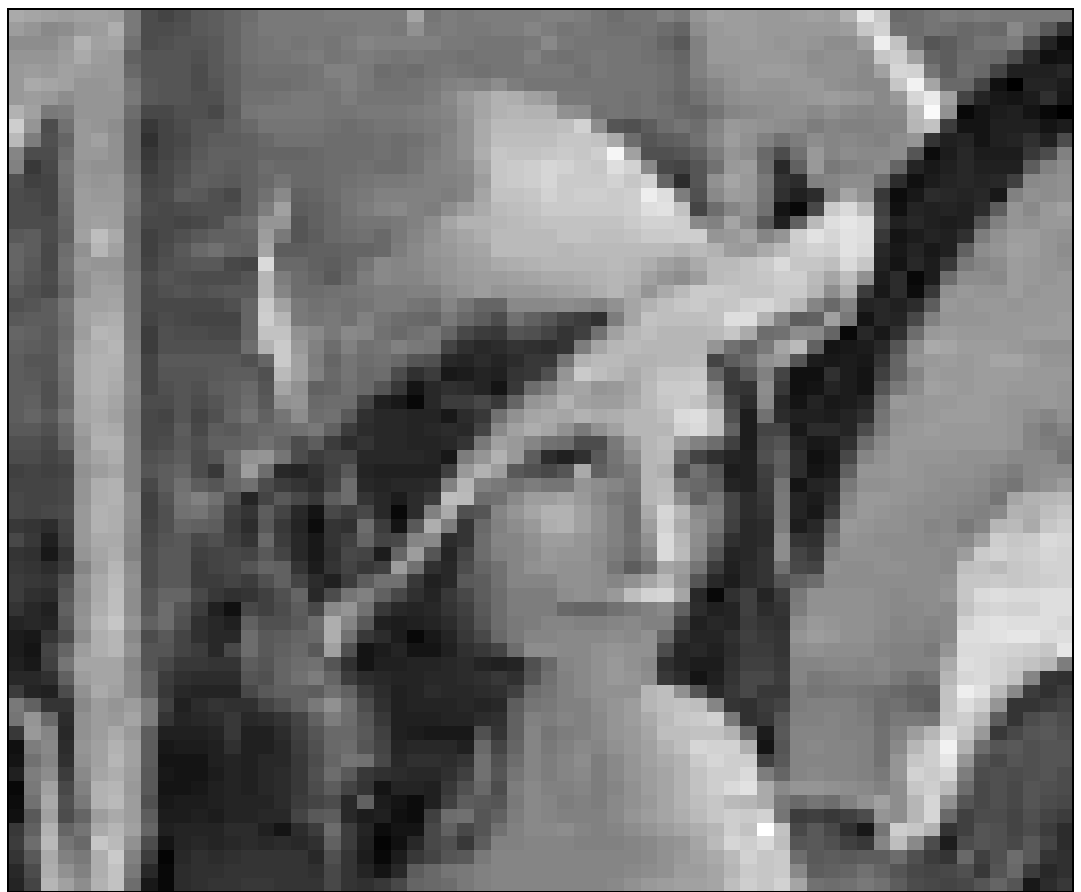
\includegraphics[width=\textwidth]{img/img_30_psnr}
				\small{psnr $\approx 30$}
				\label{psnr_30}
		\end{minipage}%
	}%
		\caption{Examples of images at different Signal to Noise ratio}
		\label{img_examples}
\end{figure}

\begin{figure}[h!]
	\makebox[\textwidth][c]{%
		\begin{minipage}[t]{0.7\textwidth}
			\centering
			\includegraphics[width=\textwidth]{img/sigma_without_prec}
			\caption{Variations of Sigma without preconditioner (tol = 
0.001, no scaling, no removal of scales)}
			\label{fig:no_prec}
		\end{minipage}%
		\qquad
		\begin{minipage}[t]{0.7\textwidth}
			\centering
			\includegraphics[width=\textwidth]{img/sigma_with_prec}
			\caption{Variations of Sigma with preconditioner (tol = 
0.001, no scaling, no removal of scales)}
			\label{fig:prec}
		\end{minipage}%
	}%
\end{figure}

To test how the aforementioned adjustments affect the performance of the 
denoising algorithm I calculate the signal to noise ratio (PSNR) for 
each iteration of conjugate gradient. All the data shown has been 
collected for three different values of sigma (0.05, 0.1 and 0.15) in 
relation to the images defined on [0,1]. Most figures show only data for 
one value of sigma (0.1) except for cases where there are remarkable 
differences in behaviour.  Similarly for the two systems solved during 
every iteration of the Gibbs sampler, the figures are only showing the 
data for the system solving for $\textbf{u}_{\mu}$, except for cases 
where differences in behaviors between the two systems warrant a special 
mention. The reason behind this decision is that its much simpler to 
reason about the signal to noise ratio when every value appears in 
continuation of the last. Had both values been plotted, they would 
either have been shown interleaven in the plot making it harder to read, 
or next to each other in separate graphs taking up twice the space for 
what turned out to be almost identical information. $\textbf{u}_{\mu}$ 
was chosen because the Rao-Blackwellised Gibbs sampling samples the 
denoised image exclusively from $\textbf{u}_{\mu}$.  

All tests shown were conducted with a burn-off limit of 3000 conjugate 
gradient iterations, and a final cut-off after 10000 conjugate gradient 
iterations in total.  This means that the psnr for $\textbf{u}_{\mu}$ 
has been noted down for about 5000 iterations.  Except when explicitly 
stated, all plots show the first 5000 iterations on the x-axis. The 
y-axis however is scaled and cropped to highlight particular details.

In order to evaluate what different levels of signal to noise ratio 
translates to in image quality, figure \ref{img_examples} showcases some 
examples for values typically encountered during the experiments. To 
compare the signal to noise ratio of an imaged with added gaussian noise 
at a standard deviation of 0.05, 0.1 or 0.15  (for an image defined on 
[0,1]) is respectively $26.3, \, 20.0$ and $16.5$ approximately. 

\begin{figure}[h!]
	\centering
	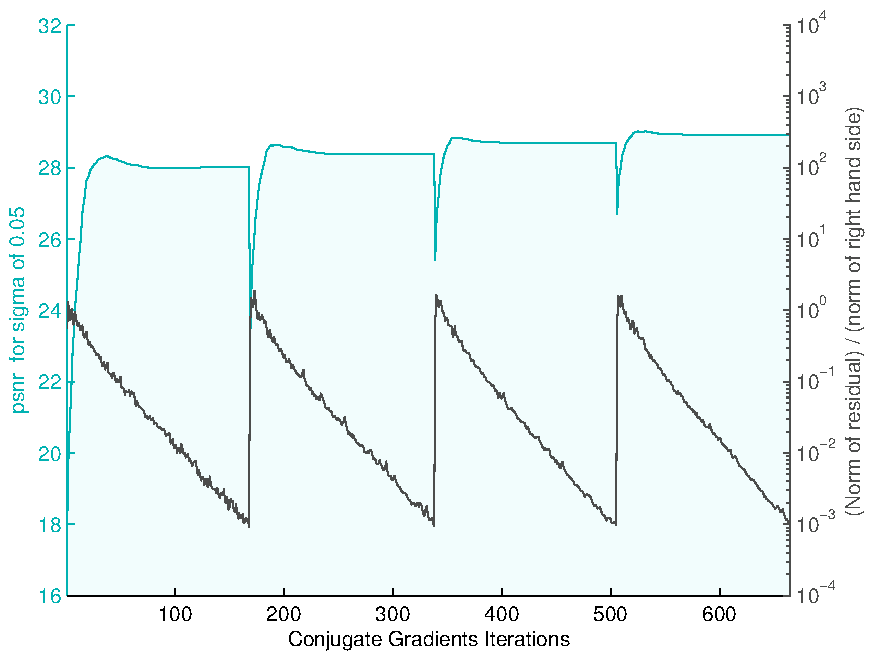
\includegraphics[width=0.7\textwidth]{img/normal_zoom}
	\caption{Four iterations plotted with residual norm (sigma = 0.05, 
tol = 0.001, no scaling, no removal of scales, with preconditioner}
	\label{fig:res_error}
\end{figure}


\begin{figure}[h!]
	\makebox[\textwidth][c]{%
		\begin{minipage}[t]{0.7\textwidth}
			\centering
			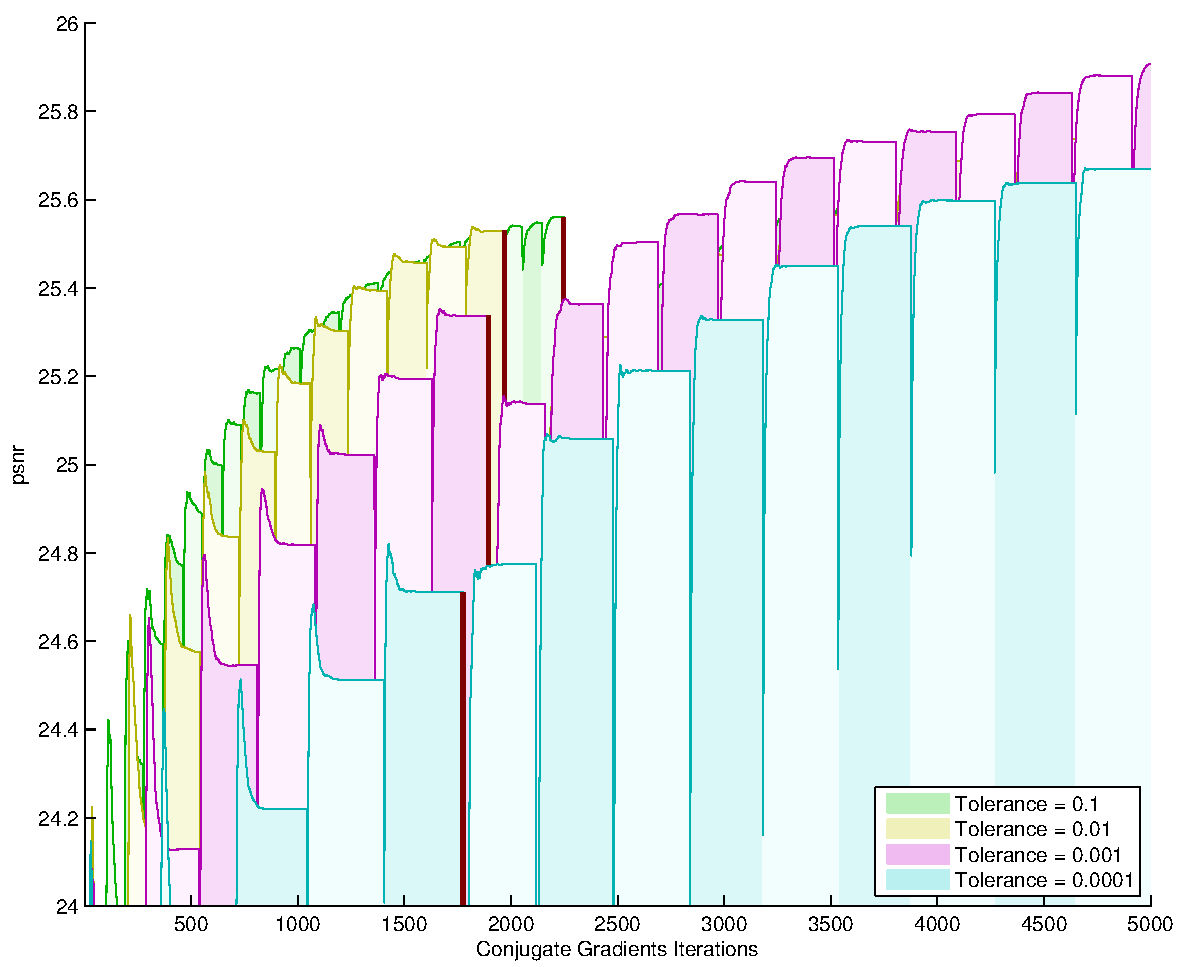
\includegraphics[width=\textwidth]{img/tolerance_overview}
			\caption{Variation of Tolerance at sigma = 0.1 (no scaling, 
no removal of scales, with preconditioner)}
			\label{fig:tolerance}
		\end{minipage}%
		\qquad
		\begin{minipage}[t]{0.7\textwidth}
			\centering
			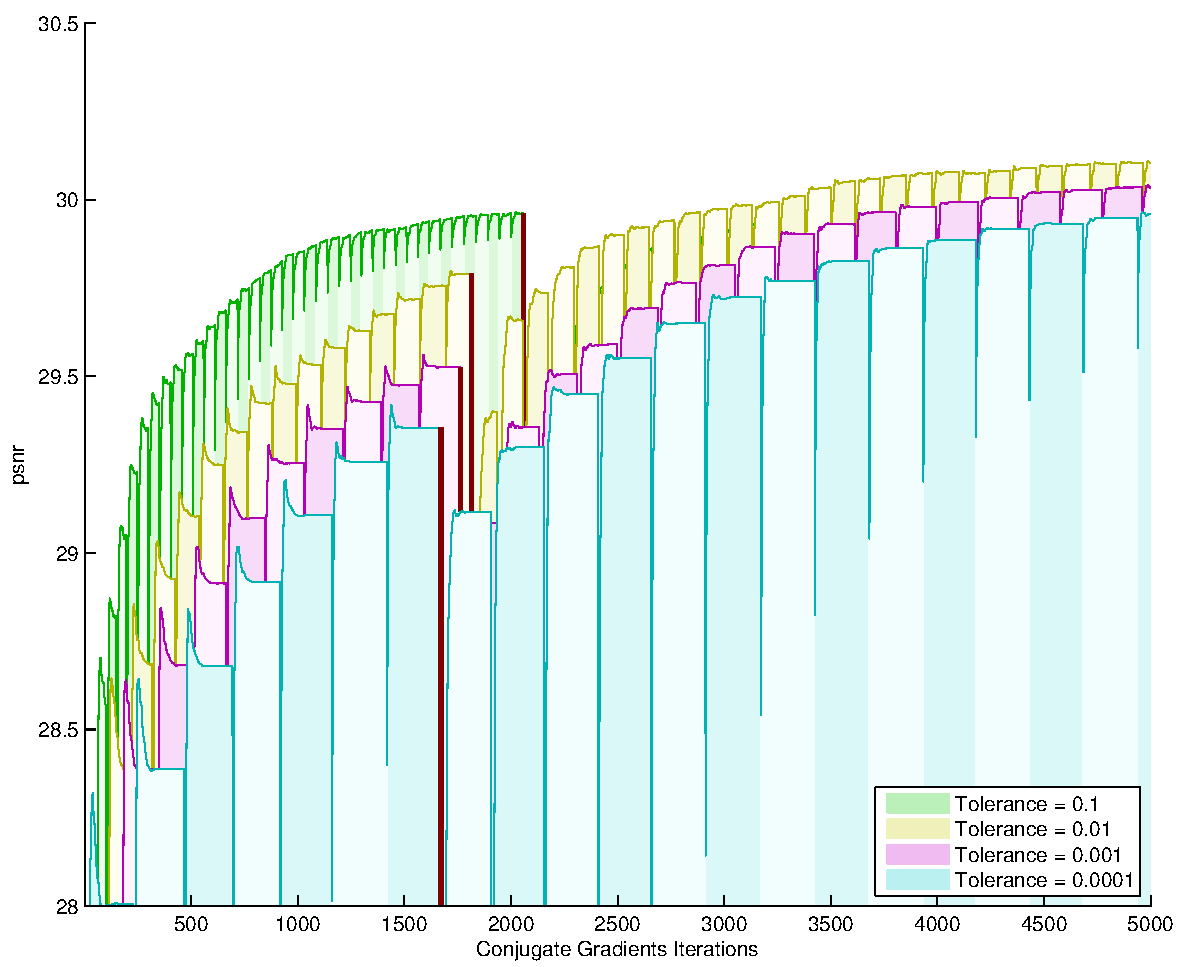
\includegraphics[width=\textwidth]{img/tolerance_low_sigma}
			\caption{Variation of Tolerance at sigma = 0.05 (no scaling, 
no removal of scales, with preconditoner)}
			\label{fig:tol_high_sigma}
		\end{minipage}%
	}%
\end{figure}

Figure \ref{fig:no_prec} shows a run with the preconditioner disabled 
for three values of sigma.  The area underneath each line has been 
shaded in alternating colors to indicate the duration of each conjugate 
gradient run. At the burn-off where the initial samples are discarded, 
the plot is marked with a red vertical line. The burn-off happens when a 
conjugate gradient run finishes and has surpassed a certain amount of 
iterations, which means it doesn't happen at the exact same iteration 
for all runs.  From the plot we can observe how the values of $\sigma$ 
influence the signal to noise ratio as well as the amount of iterations 
for each conjugate gradient run. For $\sigma = 0.05$ the mean amount of 
iterations is 222.7, while it is respectively 447.6 and 489.8 for 
$\sigma = 0.1$ and $\sigma = 0.15$. When we active the preconditioner as 
illustrated in figure
\ref{fig:prec} the means of iterations are 184.8, 274.0, 318.8 for 
$\sigma = 0.05, 0.1, 0.15$ respectively. However the signal to noise 
ratio is almost identical iteration for iteration with the 
preconditioner being on average 0.3\% better for $\sigma = 0.05$ (with a 
sample variance of 0.00047 over 5000 samples) than the case without 
preconditioner. For $\sigma = 0.1$ and $0.15$ the means are 1\% higher 
and 1\% lower respectively.

If we take a closer look in figure \ref{fig:res_error} we can see how 
each iteration of conjugate gradient using preconditioner starts out 
with a low signal to noise ratio but quickly reaches a maximum before it 
settles.  The exponential decay of the norm of the residual is plotted 
on top of the graph on a logarithmic scale, showing that no real change 
in the signal to noise ratio takes place after the norm of the residual 
passes below 0.1.


\begin{figure}[h]
		\centering
		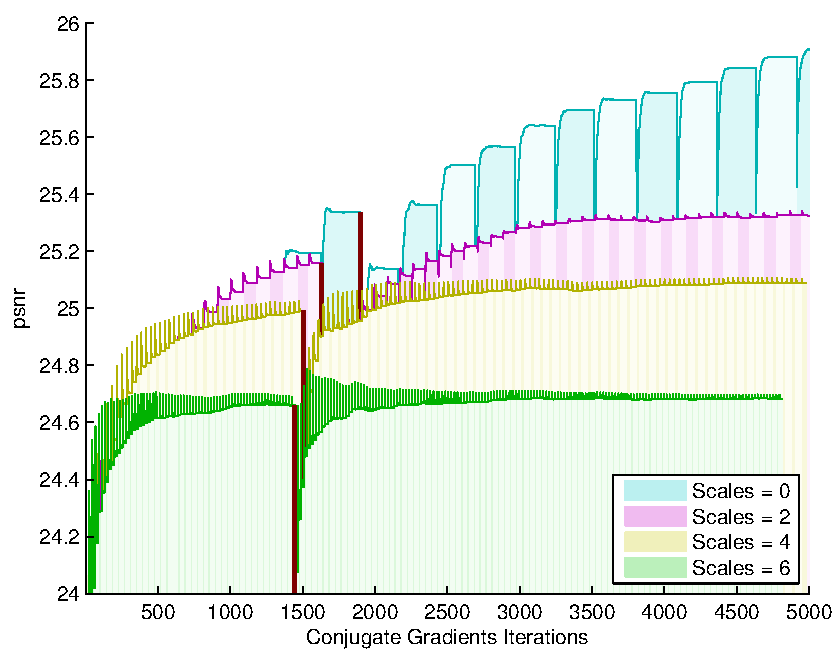
\includegraphics[width=0.7\textwidth]{img/rem_scales_overview}
		\caption{Removal of scales at sigma = 0.1 (tol = 0.001, no 
scaling, with preconditioner)}
		\label{fig:rem_scales}
\end{figure}%

The effects of lowering the tolerance can be seen in figure 
\ref{fig:tolerance} and \ref{fig:tol_high_sigma}. For $\sigma = 0.1$ in 
figure \ref{fig:tolerance} the higher tolerance improves the steepness 
of the curve, but comes at a cost. Ultimately the signal to noise ratio 
of the more exact cases with tolerance $= 0.001$ or $0.0001$ surpasses 
the higher tolerances. For the smallest measured standard deviation 
($\sigma = 0.05$) this isn't the case as the tolerance of 0.01 still 
maintain a signal to noise ratio 0.3\% better than that of the tolerance 
of 0.001 after 5000 iterations.


Figure \ref{fig:rem_scales} depicts the effect of removing the more 
extreme scales. As expected the conjugate gradient iterations become a 
lot quicker, but it comes at the cost of decreased performance. A 
similar behavior can be seen in figure \ref{fig:scaling}. Here the 
scales have been removed two by two, greatly improving the speed of the
conjugate gradient algorithm but at the cost of quality. The more scales 
removed, the earlier the plots converge toward a constant value. In 
figure \ref{fig:colormap_scales} a more detailed account of the same 
data can be seen.  A grid is made by plotting the maximum signal to 
noise ratio for each interval of a 100 iterations, as the scale factor 
is varied from 1 to 0.1 in steps of 0.05.

\begin{figure}[h]
	\makebox[\textwidth][c]{%
		\begin{minipage}[t]{0.6\textwidth}
			\centering
			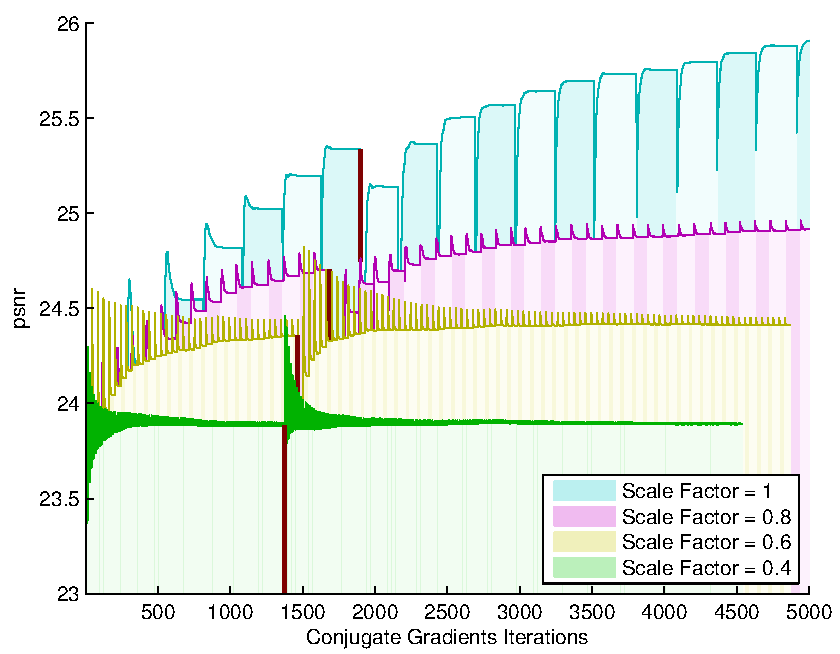
\includegraphics[width=\textwidth]{img/scaling_overview}
			\caption{Variation of Scales at sigma = 0.1 (tol = 0.001, no 
removal of scales, with preconditioner)}
			\label{fig:scaling}
		\end{minipage}%
		\qquad
		\begin{minipage}[t]{0.6\textwidth}
			\centering
			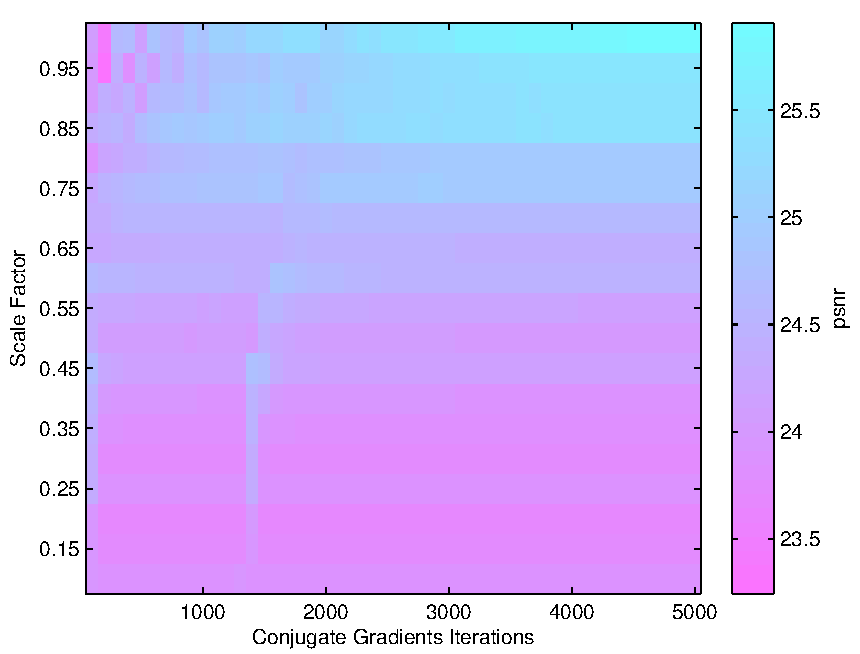
\includegraphics[width=\textwidth]{img/Scaling_heatmap}
			\caption{Variation of Scales at sigma = 0.1 (tol = 0.001, no 
removal of scales, with preconditioner)}
			\label{fig:colormap_scales}
		\end{minipage}%
	}%
\end{figure}


\section{Discussion}

In order to interpret the results, it's important to keep in mind that 
the model used was optimized for the original scales. This means that 
removing scales or changing them comes with the added cost of running 
the model in an environment it hasn't been optimized for. It might not 
be impossible to learn another model with smaller scales that perform as 
well as the current even if the results don't show greater rates for 
reduced scales.  Furthermore these results are based on simulations run 
on a single image and as such prone to fluctuations and issues that 
might not show up were more images considered.

In this light we can see from modifying the scales that the conjugate 
gradient algorithm does indeed converge faster when the scales are less 
extreme, a useful lesson if we are to learn our own scales later on.  

For applications where speed is more important than a few percents gain 
in signal to noise ratio, adjusting the tolerance of the conjugate 
gradient algorithm can prove useful. Higher tolerance rates have shown 
to provide faster climbs but tend to come at the price of a lower global 
maximum of signal to noise ratio. However for low noise applications the 
costs associated with increasing the tolerance are reduced. The gains in 
speed are relatively small though.

Although the preconditioner does not perform very well, the improvements 
it brings using it comes for free, in the sense the we get both a better 
conjugate gradient convergence and a better overall performance for most 
cases, albeit with a very small margin.

In \citep{uwe} a lot of weight is put on the fact that the prior 
resembles the long tailed distributions seen in natural images. It would 
be interesting to see if there is space for compromise between the 
realistic but slow distributions and their fast but inaccurate 
counterparts.


% Talk about
\section{Conclusion}

In order to improve the efficiency of the Fields of Experts framework I 
implemented a denoising algorithm using the framework in combination 
with the conjugate gradient algorithm. Based on this implementation I 
demonstrated that adjusting the scales of the auxiliary variable Gibbs 
sampler to create a prior with a smaller long tail does increase 
conjugate gradient convergence, but doesn't improve overall performance.  
Moreover, I showed that adjusting the tolerance of the conjugate 
gradient algorithm can improve performance, especially for low 
variances.

% Bibliography
\bibliographystyle{plain}
\bibliography{report}

\end{document}
